\documentclass[a4paper, 11pt]{article}
\usepackage{comment}
\usepackage{lipsum} 
\usepackage{fullpage} %cambiar margen
\usepackage[a4paper, total={7in, 10in}]{geometry}

\usepackage{amssymb,amsthm} 
\usepackage{amsmath}
\newtheorem{theorem}{Theorem}
\newtheorem{corollary}{Corollary}
\usepackage{graphicx}
\usepackage{tikz}
\usetikzlibrary{arrows}
\usepackage{verbatim}
%\usepackage[numbered]{mcode}
\usepackage{float}
\usepackage{tikz}
\usetikzlibrary{shapes,arrows}
\usetikzlibrary{arrows,calc,positioning}
\usepackage{mathpazo} %tipo de letra 
\usepackage[utf8]{inputenc} %codificación
\usepackage[T1]{fontenc} %digitación de tildes y ñ
\usepackage[spanish]{babel} %paquete de soporte español

\tikzset{
	block/.style = {draw, rectangle,
		minimum height=1cm,
		minimum width=1.5cm},
	input/.style = {coordinate,node distance=1cm},
	output/.style = {coordinate,node distance=4cm},
	arrow/.style={draw, -latex,node distance=2cm},
	pinstyle/.style = {pin edge={latex-, black,node distance=2cm}},
	sum/.style = {draw, circle, node distance=1cm},
}
\usepackage{xcolor}
\usepackage{mdframed}
\usepackage[shortlabels]{enumitem}
\usepackage{indentfirst}
\usepackage{hyperref}

\usepackage{listings}
\lstset{literate=
  {á}{{\'a}}1
  {é}{{\'e}}1
  {í}{{\'i}}1
  {ó}{{\'o}}1
  {ú}{{\'u}}1
  {Á}{{\'A}}1
  {É}{{\'E}}1
  {Í}{{\'I}}1
  {Ó}{{\'O}}1
  {Ú}{{\'U}}1
  {ñ}{{\~n}}1
  {ü}{{\"u}}1
  {Ü}{{\"U}}1
}

\lstdefinestyle{customc}{
  belowcaptionskip=1\baselineskip,
  breaklines=true,
  frame=L,
  xleftmargin=\parindent,
  language=Python,
  showstringspaces=false,
  basicstyle=\footnotesize\ttfamily,
  keywordstyle=\bfseries\color{green!40!black},
  commentstyle=\itshape\color{purple!40!black},
  identifierstyle=\color{blue},
  stringstyle=\color{orange},
}

\lstdefinestyle{customasm}{
  belowcaptionskip=1\baselineskip,
  frame=L,
  xleftmargin=\parindent,
  language=[x86masm]Assembler,
  basicstyle=\footnotesize\ttfamily,
  commentstyle=\itshape\color{purple!40!black},
}

\lstset{escapechar=@,style=customc}



\renewcommand{\thesubsection}{\thesection.\alph{subsection}}

\newenvironment{problem}[2][Ejercicio]
{ \begin{mdframed}[backgroundcolor= red!50] \textbf{#1 #2} \\}
	{  \end{mdframed}}

% Define solution environment
\newenvironment{solution}
{\textcolor{blue}{\textbf{\textit{Solución:\\\noindent}}}}


\renewcommand{\qed}{\quad\qedsymbol}

% \\	
\begin{document}
	\noindent
	%%%%%%%%%%%%%%%%%%%%%%%%%%%%%%%%%%%%
	
	\begin{minipage}[b][1.2cm][t]{0.8\textwidth}
		\large\textbf{César Isaí García Cornejo} \hfill \textbf{Tarea 11}  \\
		cesar.cornejo@cimat.mx \hfill \\
		\normalsize Computo Científico \hfill Semestre 3\\
	\end{minipage}
	
	\hspace{14.4cm}
	\begin{minipage}[b][0.03cm][t]{0.12\linewidth}
		
		\vspace{-2.2cm}
		%%%La Ruta dependerá de donde este alojado el main y la imagen
		
\includegraphics[scale=0.3]{Figures/EscudoCimat.png}
	\end{minipage}
	
	\noindent\rule{7in}{2.8pt}
	
	%%%%%%%%%%%%%%%%%%%%%
	%%%%%%%%%%%%%%%%%%%%%%%%%%%%%%%%%%%%%%%%%%%%%%%%%%%%%%%%%%%%%%%%%%%%%%%%%%%%%%%%%%%%%%%%%%%%%%%%%%%%%%%%%%%%%%%%%%%
	% Problem 1
	%%%%%%%%%%%%%%%%%%%%%%%%%%%%%%%%%%%%%%%%%%%%%%%%%%%%%%%%%%%%%%%%%%%%%%%%%%%%%%%%%%%%%%%%%%%%%%%%%%%%%%%%%%%%%%%%%%%%%%%%%%%%%%%%%%%%%%%%
	\setlength{\parskip}{\medskipamount}
	\setlength{\parindent}{0pt}
%/////////// Ejercicio 1 /////////////////

\begin{problem}{1}
    Usando la base de datos MNIST realice lo siguiente y explique cada decisión tomada:
    \begin{enumerate}
        \item Diseñe una red neuronal de una sola capa oculta para la clasificación de las imágenes. Use una función de pérdida predefinida. 
        \item Entrene la red neuronal 
        \item Presente la matriz de confusión (Confusion matrix),
        \item Describa que es la precisión y la exhaustividad (precisión and recall) y calculelo a partir de su matriz de confusión 
    \end{enumerate}
\end{problem}

\begin{solution} 
    Los códigos se encuentran en \href{https://colab.research.google.com/drive/1KPaXDHSXw70dSOGzQkdSyyUeZKSXxZWm?usp=sharing}{\textcolor{blue} {aquí}}.

    Procedemos a hacer cada paso en el siguiente orden:
    \begin{enumerate}
        \item Cargar la base de datos MNIST (entrenamiento y prueba)
        \item Definir la red neuronal convolucional
        \item Definir una función de perdida.
        \item Entrenar la red con los datos de entrenamiento
        \item Probar la red con los datos de prueba.
    \end{enumerate}

    Cargamos la base MNIST usando \textit{torchvision}. La salida de la base de datos de torchvision son imagenes PILImages de rango [0,1]. Transformamos los datos en tensores normalizados de rango [-1,1].

    De igual forma con pytorch podemos construir la red neuronal de una sola capa, para ello observese en el código siguiente que se aplano la imagen en un vector, dado que la imagen es de $28 \times 28$ luego la entrada será de una capa de 784 neuronas. La capa de enmedio se diseño para tener 64 neuronas y finalmente la capa de salida tiene 10 neuronas ya que se desea clasificar para 10 clases que son cada uno de los dígitos.
    \begin{lstlisting}
class Net(nn.Module):
    def __init__(self):
        super().__init__()
        self.fc1 = nn.Linear(28 * 28, 64)  # Capa oculta con 64 neuronas
        self.relu = nn.ReLU()
        self.fc2 = nn.Linear(64, 10)  # Capa de salida con 10 neuronas

    def forward(self, x):
        x = torch.flatten(x, 1) # flatten all dimensions except batch
        x = F.relu(self.fc1(x))
        x = F.relu(self.fc2(x))
        return x

    \end{lstlisting}

Tomemos 4 elementos de la base de datos con fines explorativos
\begin{figure}[H] 
    \centering 
    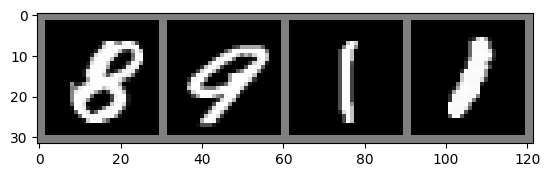
\includegraphics[width = 10 cm]{Figures/MNISTbase.png} 
    \caption{Grafica de 4 elementos aleatorios en la base MNIST}
    \label{Fig. 1.01}
\end{figure} 

La clase correspondiente es el output:
\begin{lstlisting}
    Ocho  Nueve Uno   Uno  
\end{lstlisting}

Empíricamente observamos que el número de épocas apropiado que disminuye el error de predicción es 6. Luego, entrenamos la red neuronal con 6 épocas. La función de activación es la función ReLu y la función de costos es la entropía cruzada a la cuál se optimiza con descenso de gradiente estocástico con momento.

Luego, con la base de prueba medimos la precisión de dicha red para la clasificación que obtuvo un valor de: 96\%.

Finalmente, la matriz de confusión es 
\begin{figure}[H] 
    \centering 
    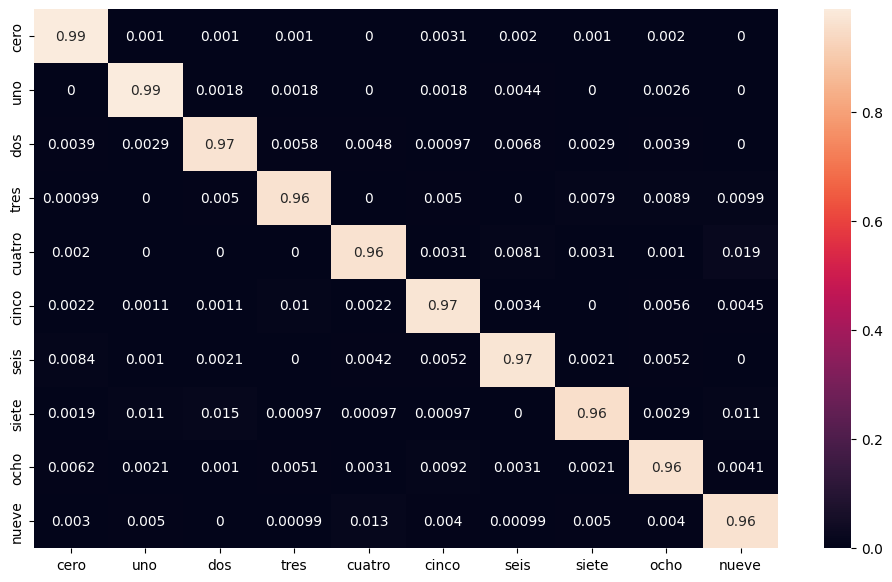
\includegraphics[width = 14 cm ]{Figures/confusionMNIST.png} 
    \caption{Matriz de confusión para la clasificación de la red neuronal entrenada con los datos de prueba en la base de datos MNIST.}
    \label{Fig. 1.02}
\end{figure}  

Observamos que es un excelente clasificador, pues la diagonal tiene valores por encima de 96\% de precisión para cada dígito.

En el contexto de reconocimiento de patrones, se denomina precisión como a la fracción de instancias recuperadas que son relevantes, mientra que la exhaustividad es la fracción de instancias relevantes que han sido recuperadas. Tanto la precisión como la exhaustividad son entendidas como medidas de la relevancia \cite{wiki}.

La precisión es una proporción entre el número de documentos relevantes recuperados entre el número de documentos recuperados.
\begin{align*}
    \text{Precisión} = \frac{|\{documentos\:\: relevantes\}\cap \{ documentos\:\: recuperados\}| }{\{ documentos\:\: recuperados\}}
\end{align*}

La exhaustividad se emplea en menor medida que la precisión. Esta proporción viene a expresar la proporción de documentos relevantes recuperados comparado con el total de documentos que son relevantes.
\begin{align*}
    \text{Exhaustividad} = \frac{|\{documentos\:\: relevantes\}\cap \{ documentos\:\: recuperados\}|}{\{documentos\:\: relevantes\}}
\end{align*}



De la matriz de confusión se deduce la precisión y la exhaustividad 
\begin{lstlisting}
Precisión: 0.9698
Exhaustividad (Recall): 0.9698
\end{lstlisting}
lo que concluye el ejercicio.

\end{solution}

\begin{problem}{2} 
    Usando la base de datos Fashion MNIST realice o siguiente y explique cada decisión tomada:
    \begin{enumerate}
        \item Diseñe una red neuronal de dos capas ocultas para la clasificación de las imágenes, cada una con diferente función de activación y use una función de pérdida en la que el error de clasificar mal un calzado sea el doble que el resto de prendas.
        \item Entrene la red neuronal
        \item Presente la matriz de confusión (Confusion matrix).
    \end{enumerate}
\end{problem}

\begin{solution} 

    Cargamos los datos usando torchvision cargando FashionMNIST, tenemos images de 28*28 de un solo canal. Análogo al ejercicio previo, diseñamos una red neuronal completamente conectada, es decir es necesario aplanar la imagen en un vector 28*28. Luego, la primer capa oculta se propone de 256 capas, la segunda capa se propone de 64 capas y la capa de salida es de 10 neuronas, ya que hay 10 clases. Tomamos dos funciones de activación, la función ReLu para la primera capa, la función sigmoide para la segunda y para la capa de salida nuevamente usamos la función ReLu.

    Con fines explorativos mostramos cuatro elementos de la base de datos Fashion MNIST tomados aleatoriamente.
    \begin{figure}[H] 
        \centering 
        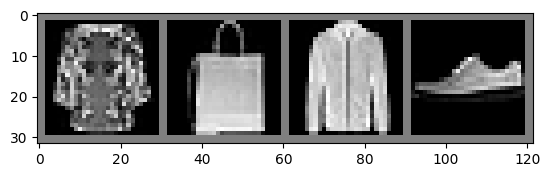
\includegraphics[width = 10 cm]{Figures/FMNISTbase.png} 
        \caption{Grafica de 4 elementos aleatorios en la base FashionMNIST.}
        \label{Fig. 2.01}
    \end{figure} 
    donde cada elemento se muestra con la clase
    \begin{lstlisting}
    Shirt Bag   Coat  Sneaker
    \end{lstlisting}

    Veamos en el código siguiente la construcción de la red neuronal
    \begin{lstlisting}
class Net(nn.Module):
    def __init__(self):
        super().__init__()
        self.fc1 = nn.Linear(28 * 28, 256)  # Capa oculta con 256 neuronas
        self.fc2 = nn.Linear(256, 64)  # Capa oculta con 64 neuronas
        self.fc3 = nn.Linear(64, 10)  # Capa de salida con 10 neuronas

    def forward(self, x):
        x = torch.flatten(x, 1) # flatten all dimensions except batch
        x = F.relu(self.fc1(x))
        x = F.sigmoid(self.fc2(x))
        x = F.relu(self.fc3(x))
        return x
    \end{lstlisting}

    Para la función de perdida, damos un vector de pesos donde a cada clase le asocia peso 1 a excepción de la última clase que tiene peso 2, es decir la clase de \textit{Ankle Boot}.

    Luego, dichos pesos se mandan a llamar como argumento para la función de perdida de entropía cruzada. Es decir, simplemente la implementación es
    \begin{lstlisting}
        weight = torch.tensor([1.0] * 9 + [2.0])  # Asignar peso 2.0 a la última clase
        criterion = nn.CrossEntropyLoss(weight=weight)
        optimizer = optim.SGD(net.parameters(), lr=0.001, momentum=0.9)
    \end{lstlisting}
    Nótese que el peso es concatenación, obteniendo un vector de 10 elementos.
    
    Ahora, tras varios experimentos concluimos que el número de épocas ideales son 8. Entrenando la red neuronal y haciendo la prueba de la precisión con los datos de prueba se obtiene que la red neuronal clasifica con un 86\% de precisión.

    Podemos ver los detalles de la clasificación con los datos de prueba en la matriz de confusión siguiente
    \begin{figure}[H] 
        \centering 
        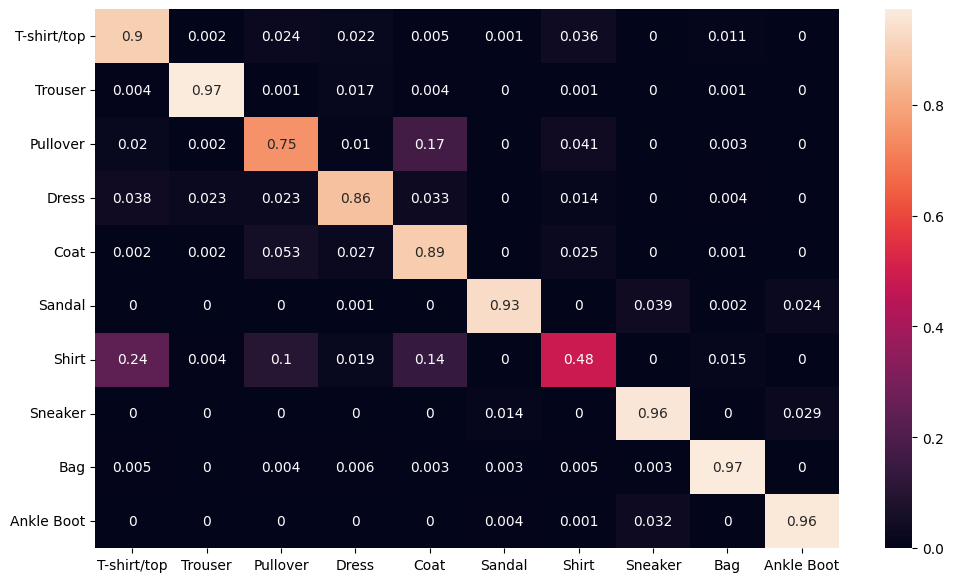
\includegraphics[width = 14 cm]{Figures/confusionFMNIST.png} 
        \caption{Matriz de confusión para la clasificación de la red neuronal entrenada con los datos de prueba en la base de datos MNIST.}
        \label{Fig. 2.02}
    \end{figure} 
    
    Podemos ver que tiene valores muy altos en la diagonal, lo que significa que la mayoría de las prendas las consigue clasificar con precisión aceptable. Sin embargo, prendas como \textit{Shirt} tiene problemas para decidir con precisión, de hecho vemos que el clasificador confunde \textit{Shirt} con \textit{T-Shirt} y también con \textit{Coat}.











  
\end{solution}

\begin{problem}{3} 
    Con la base de datos CIFAR-10 realice lo siguiente:
    \begin{enumerate}
        \item Diseñe una red neuronal de una capa oculta completamente conectada de al menos 10,000 neuronas para la clasificación de las imágenes.
        \item Entrene la red neuronal 
        \item Presenta la matriz de confusión (Confusion matrix)
        \item Entrene una segunda red neuronal usando la estructura de LeNet5 
        \item Presente la matriz de confusión (Confusion matrix)
        \item Compare ambas redes. Para esta comparación será necesario que al menos presenta las curvas de error de entrenamiento y predicción para ambas redes, los tiempos de entrenamiento y que tome en cuenta las matrices de confusión.
    \end{enumerate}
\end{problem}

\begin{solution} 

    Observemos que la base de datos se compone de imagenes a color, es decir cada imagen tiene tres canales. Luego, se tiene que ajustar los parámetros en el diseño de la red y en la transformación de forma que sea compatible con el formato. 

    \begin{figure}[H] 
        \centering 
        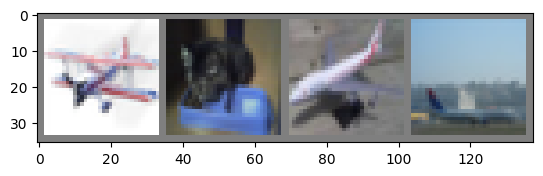
\includegraphics[width = 10 cm]{Figures/CIFARbase.png} 
        \caption{Grafica de 4 elementos aleatorios en la base CIFAR-10.}
        \label{Fig. 3.01}
    \end{figure} 

    La primera estructura de red se compone de una capa completamente conectada con 10000 neuronas. 

    Entrenamos la red neuronal con 50 épocas y un batch size de 512, luego gráficamos la perdida de entrenamiento y de predicción obteniendo 
    \begin{figure}[H] 
        \centering 
        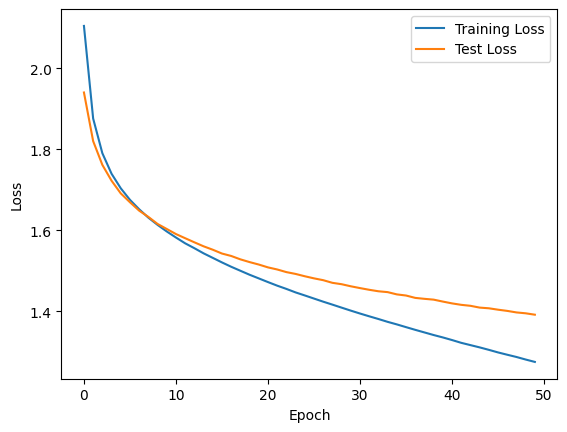
\includegraphics[width = 10 cm]{Figures/curvaerrorCIFAR_01.png  } 
        \caption{Grafica de la función de perdida de entrenamiento y predicción para la red neuronal de 10000 neuronas en una capa oculta.}
        \label{Fig. 3.02}
    \end{figure} 

    Como vemos en la figura anterior, la perdida disminuye con cada época. Por tanto, nos quedamos con la red al máximo de épocas que es 50. Con esto vemos en el código que dicha red tiene una precisión con los datos de prueba del 51\%.

    La matriz de confusión de la red neuronal como clasificador es 
    \begin{figure}[H] 
        \centering 
        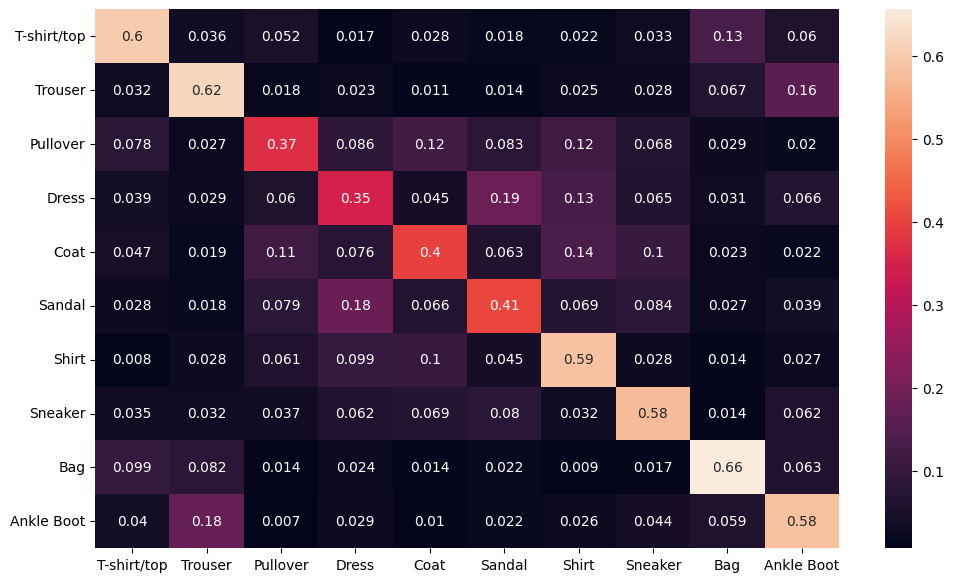
\includegraphics[width = 14 cm]{Figures/confusionCIFAR_01.png} 
        \caption{Matriz de confusión para la red neuronal de una capa oculta con 10000 neuronas.}
        \label{Fig. 3.03}   
    \end{figure} 


    En efecto vemos que en cada elemento se tiene una clasificación cercana al 50\%. Lo que no es un excelente clasificador pero es mejor que uno aleatorio con 10\% de precisión.

    Luego, para la segunda estructura que es la correspondiente a la estructura LeNet 5, entrenamos la red neuronal con 40 épocas obteniendo la siguiente grafica de la función de perdida por época
    \begin{figure}[H] 
        \centering 
        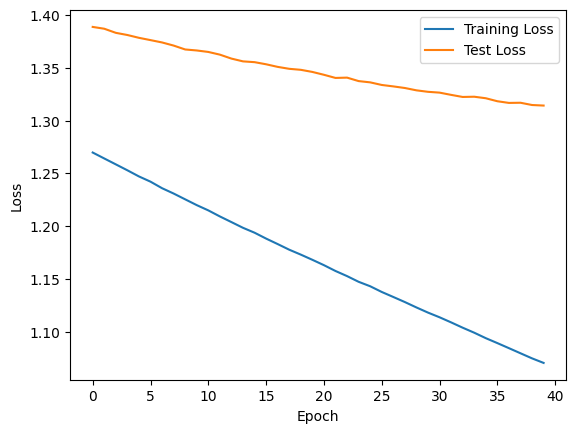
\includegraphics[width = 10 cm]{Figures/curvaerrorCIFAR_02.png} 
        \caption{Gráfica de la función de perdida para la red neuronal de LeNet 5 con la base de datos de CIFAR-10.}
        \label{Fig. 3.04}
    \end{figure} 

    Nuevamente, vemos que la función de perdida disminuye a medida con cada época. Luego tomamos la red neuronal entrenada con 40 épocas. La precisión con los datos de prueba nos da ligeramente mayor que la red neuronal que deseamos contrastar, con un 59\% de precisión. Vemos en su matriz de confusión los errores de clasificación. 
    \begin{figure}[H] 
        \centering 
        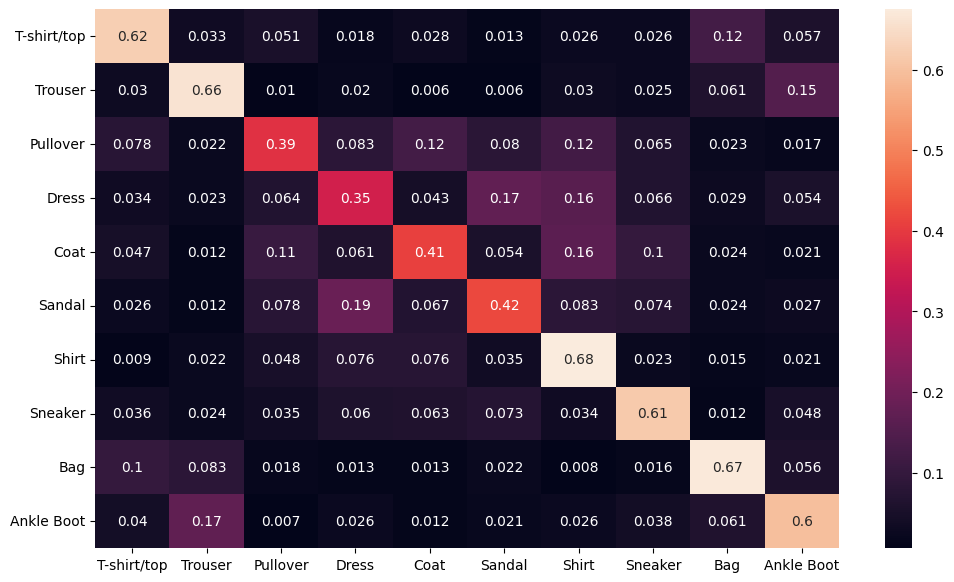
\includegraphics[width = 14 cm]{Figures/confusionCIFAR_02.png} 
        \caption{Matriz de confusión para la red neuronal LeNet 5.} 
        \label{Fig. 3.05}
    \end{figure} 

    La precisión de la red neuronal se aumenta bajando el número batch size, sin embargo algo muy bajo implica tiempos no considerables de cómputo que no bajan ni usando el GPU. 
    
    En consideraciones generales, la red LeNet5 fue mejor en precisión de prueba que la red simple sobrecargada, ya que se entreno 10 épocas menos y se obtuvo una precisión mayor a pesar de esto. 
  
\end{solution}


% \begin{problem}{4} 
%     usando la base de datos MNIST y la estructura LeNet5  realice lo siguiente:
%     \begin{enumerate}
%         \item Entrene la red neuronal
%         \item Implemente el algoritmo \textit{Deepfool} y construya un ejemplo adversario para cada una de las categorías, presente la imagen original, el ruido que añadió y la nueva imagen.
%     \end{enumerate}
% \end{problem}




\begin{thebibliography}{9}

    % \bibitem{Casella}
    % Robert, C. P., Casella, G., and Casella, G. (1999). Monte Carlo statistical methods (Vol. 2). New York: Springer.

    % \bibitem{Wasserman}
    % Wasserman, L. (2004). All of statistics: a concise course in statistical inference (p. 413). New York: Springer.
    
    \bibitem{wiki}
    Precisión y exhaustividad. 
    \url{https://es.wikipedia.org/wiki/Precisi%C3%B3n_y_exhaustividad}

    \bibitem{pytorch}
    Tutorial redes neuronales.
    \url{https://pytorch.org/tutorials/beginner/blitz/cifar10_tutorial.html}


\end{thebibliography}
      




\end{document}